\chapter{Experiments and results}
\label{chap:experiments_and_results}


	% --- META INFO START: ---

	\besk{Gode eksperimenter som motiveres og forklares, settes opp, og utføres m/resultater man diskuterer og analyserer. Det er bra å evaluere fra flere synspunkt \tcol[gray]{med flere research methods og hvis tid}}

	% --- META INFO STOP. ---


This chapter presents the experiments set up and performed in the novel synchronization simulator in Unity, as presented in Chapter \ref{chap:implementation}, for certain configurations of musical robot collectives. Effects of the individual musical robots's hyperparameters on the collective achievement and performance of achieving harmonic synchrony are presented. Some examples are hyperparameters which determines how much each musical robot will adjust itself after hearing a transmitted fire signal from a neighbouring robot; $\alpha$ for phase adjustment and $\beta$ for frequency adjustment.

The main performance scores presented in this chapter will consist of synchronization times given in simulation time (s) (i.e. how long it takes robot collectives to reach the state of harmonic synchrony if they ever do), accompanied by the respective and corresponding error rates during the belonging simulation runs (i.e. the percentage of robot collectives out of e.g. 30 runs failing to reach harmonic synchrony before the maximum time limit of e.g. 5 simulation minutes). If a musical robot collective then never reaches the target state of harmonic synchrony within the maximum time limit, this simulation run will be regarded as a ``synchronization fail'', and we will then not regard its termination time (in simulation time seconds) as \textit{harmonic synchronization time}—but simply that, that simulation run's termination time.

As previously mentioned, relating to the different robot colors like turquoise, red, and green, all robots are homogenous apartly from the visual; all individual robots have for experiments the same hyperparameters unless otherwise is explicitly stated.



\section{Data visualization}

	% --- META INFO START: ---

	\besk{Der jeg forklarer SimRun-plotsa mine som analyserer synkroniseringsruns, som jeg kun skal bruke samlet med screenshots av synkroniseringsruns før vs. etter én gang for 1) Phase sync og 2) Phase and frequency sync, og ellers bare evt. (sub-)plots av dersom det er hensiktsmessig og ikke overflødig og rotete}

	% --- META INFO STOP. ---


\section{Phase synchronization}
\label{sec:phase_sync}
This is the section where experiments attempting to synchronize for the first and simpler problem, namely synchronizing only the phases $\phi_i$ of all agents $i$, are presented and analyzed resuls for. These are then experiments where all musical robots have an equal and fixed frequency, only adjusting phases, in order to entrain to synchronize their phases to each other until reaching the target state of harmonic synchrony. Or in other words, all experiments in this phase synchronization section have the two hyperparameters shown in Table \ref{tab:phase_sync} in addition to the individual experiment hyperparameters listed.

\begin{center}
\begin{tabular}{ |c|c|c| } 
\hline
$Adj_\phi$ & $Adj_\omega$ \\
\hline
Mirollo \& Strogatz & None  \\
\hline
\end{tabular}
\captionof{table}{Phase synchronization experiments hyperparameter setup.}
\label{tab:phase_sync}
\end{center}

	\subsection{Initial validation}
	
	To see that synchronization is actually happening like intended, some relevant quantities and simulation values are recorded for a phase synchronization simulation run in Unity and displayed in \ref{}.
	
	\tcol[blue]{FYLL INN.}
	
	\subsection{Reproducing baseline results}
	
		\paragraph{Experiment setup:\nl}
		
		In order to see that our developed synchronization simulator in Unity yields more or less the same results as Nymoen's results, similar experiments as reported in their paper are performed here. These tell us whether differences in performance, in terms of synchronization times (sim s), is simply due to implementation differences, or actually because of the utilized synchronization methods and hyperparameters in question. 
		
		First off, Mirollo \& Strogatz's phase adjustment method (as presented in \ref{mirollo_strogatz_phase_adjust}) is experimented with for the initial phase ($\phi$) synchronization problem, for varying phase coupling constants $\alpha$. Hyperparameters are set in the simulator as shown in Table \ref{tab:baseline_reproducing_phase_sync_for_alpha}. Results can be seen in Figure \ref{fig:baseline_reproducing_phase_sync_for_alpha}.
		
		\begin{center}
		\begin{tabular}{ |c|c|c|c|c|c|c| } 
		\hline
		$|R|$ & $\beta$ & $t_{ref}$ & $t_f$ & $k$ & $t_{max}$ \\
		\hline
		6 & 0 & 50ms & 80ms & 8 & 5min \\
		\hline
		\end{tabular}
		\captionof{table}{Experiment hyperparameter setup.}
		\label{tab:baseline_reproducing_phase_sync_for_alpha}
		\end{center}
		
		\paragraph{Experiment results:\nl}
		
		\begin{figure}[ht!]
			\centering
			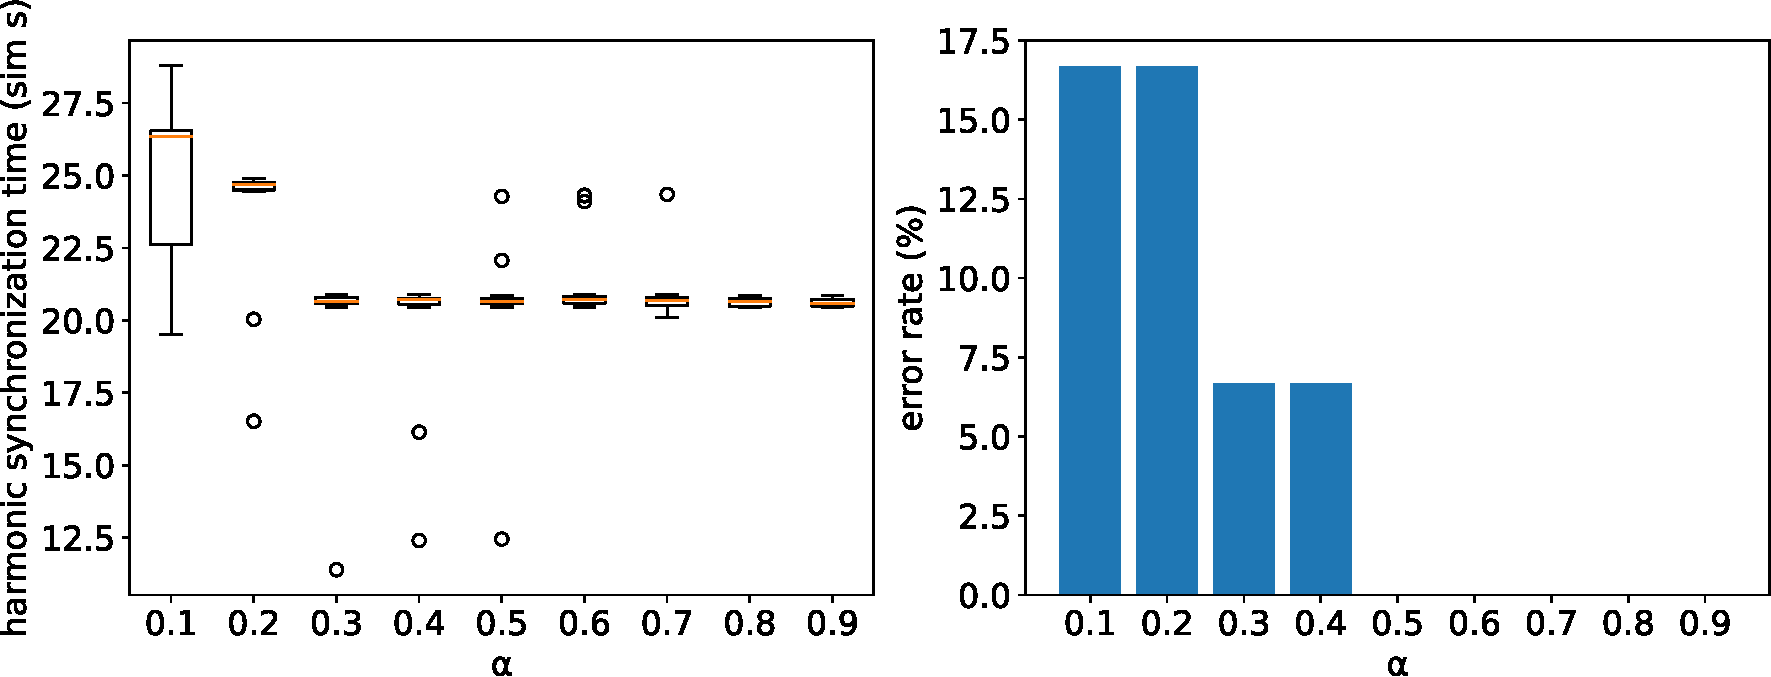
\includegraphics[width=\linewidth]{Assets/DocSegments/Chapters/ExperimentsAndResults/Figures/PerfScores/baseline_reproducing_phase_sync_for_alpha.pdf}
			\caption{Harmonic synchronization times (s) for 6 robots with initially random and unsynchronized phases but equal and fixed frequencies (1Hz), for varying phase coupling constants $\alpha$. 30 simulation runs per $\alpha$ are reported.}
			\label{fig:baseline_reproducing_phase_sync_for_alpha}
		\end{figure}
		
		\paragraph{Experiment analysis:\nl}
	
	\subsection{Hyperparameter tuning}
	
		\paragraph{Experiment setup:\nl}
		
		Here we tune the hyperparameters $\alpha$ and $t_{ref}^{dyn}$ for several robot collective sizes, according to performance scores of how long it takes robot collectives on average to achieve harmonic synchrony. Exactly these two specific hyperparameters are experimented with mostly since they empirically seem to be the most important ones to set correctly before starting the simulator; that is, in order for the robots to actually manage achieving harmonic synchrony. Additionaly, the point of K. Konishi and H. Kokame (cf. \ref{sim_env_and_hyperparams}) was also remembered.
		
		The specific values of hyperparameters to test synchronization times for were chosen based on an initial and identical but failed experiment (not reported) where the tested values for $t_{ref}^{dyn}$ were showing some interesting effects for various robot collective sizes. Simple and limited insight was also collected from trial and error in the complete beginning when trying to facilitate stable and successful simulation runs. And furthermore, after seeing results found in this thesis for $\alpha$ already, we also got some more ideas for which values of $\alpha$ could be interesting to investigate further.
		
		Other constant hyperparameters not being tuned or experimented for in this experiment are shown in Table \ref{tab:exp_phase_sync_hyperparam_tuning}. The hyperparameter tuning results, where the effects of tuning hyperparameters $\alpha$ and $t_{ref}^{dyn}$ for various musical robot collective sizes, are shown in Figure \ref{fig:phase_sync_hyperparam_tuning_experiment}. Again, since we are synchronizing for the phase ($\phi$) synchronization problem, now only phases are initially unsynchronized, and frequencies are fixed and constant (1Hz) throughout the simulation runs.
		
		\begin{center}
		\begin{tabular}{ |c|c|c|c|c| } 
		\hline
		$\beta$ & $t_f$ & $k$ & $t_{max}$ \\
		\hline
		0 & 80ms & 8 & 5min \\
		\hline
		\end{tabular}
		\captionof{table}{Experiment hyperparameter setup.}
		\label{tab:exp_phase_sync_hyperparam_tuning}
		\end{center}
		
		\paragraph{Experiment results:\nl}
		
		\begin{figure}[ht!]
		  \begin{subfigure}[b]{0.5\textwidth}
			\centering\captionsetup{width=.9\linewidth}%
			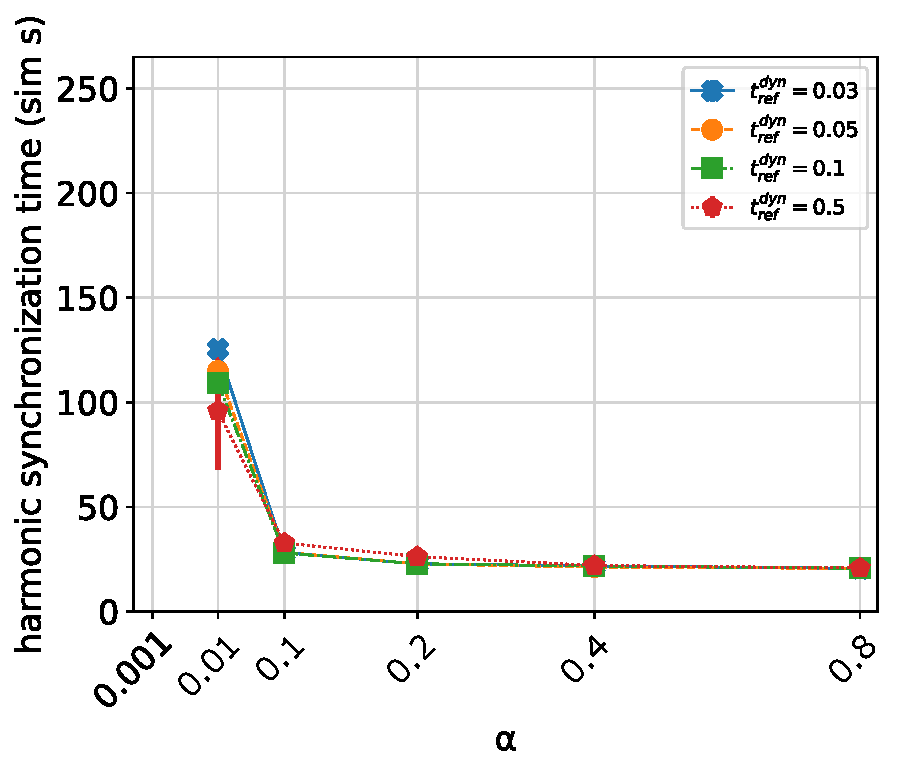
\includegraphics[width=\textwidth]{Assets/DocSegments/Chapters/ExperimentsAndResults/Figures/PerfScores/t_ref_dyn_x_alpha_hyperparamtuning_experiment_plot_collsize3.pdf}
			\caption{$|R|$ = 3.}
			\label{fig:sub:t_ref_dyn_x_alpha_collsize3}
		  \end{subfigure}
		  %
		  \begin{subfigure}[b]{0.5\textwidth}
			\centering\captionsetup{width=.9\linewidth}%
			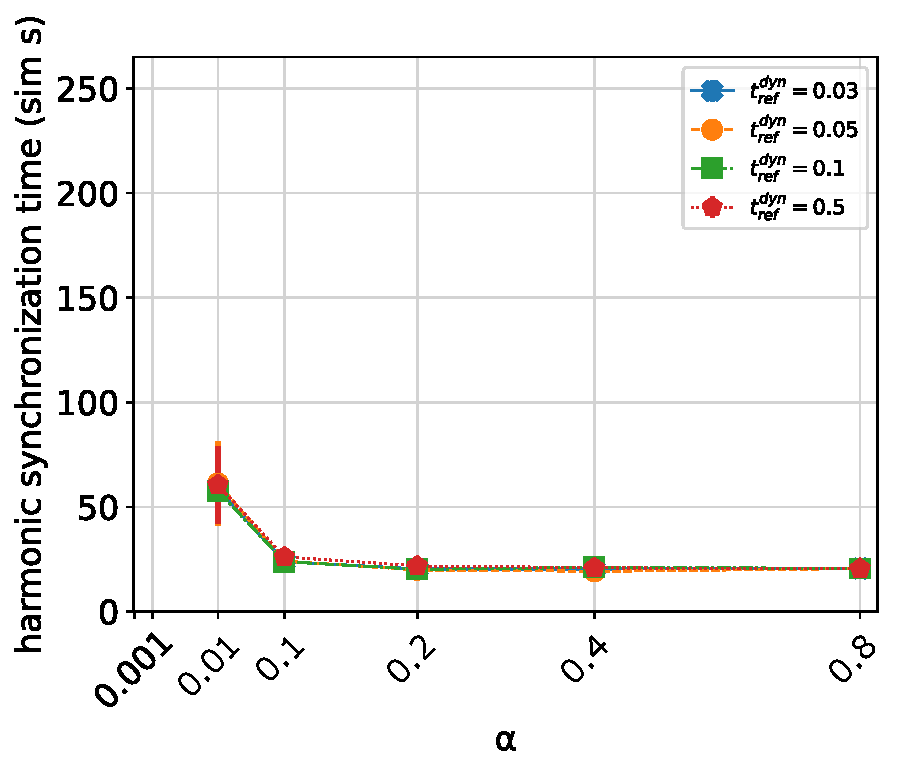
\includegraphics[width=\textwidth]{Assets/DocSegments/Chapters/ExperimentsAndResults/Figures/PerfScores/t_ref_dyn_x_alpha_hyperparamtuning_experiment_plot_collsize10.pdf}
			\caption{$|R|$ = 10.}
			\label{fig:sub:t_ref_dyn_x_alpha_collsize10}
		  \end{subfigure}
		  \begin{subfigure}[b]{0.5\textwidth}
			\centering\captionsetup{width=.9\linewidth}%
			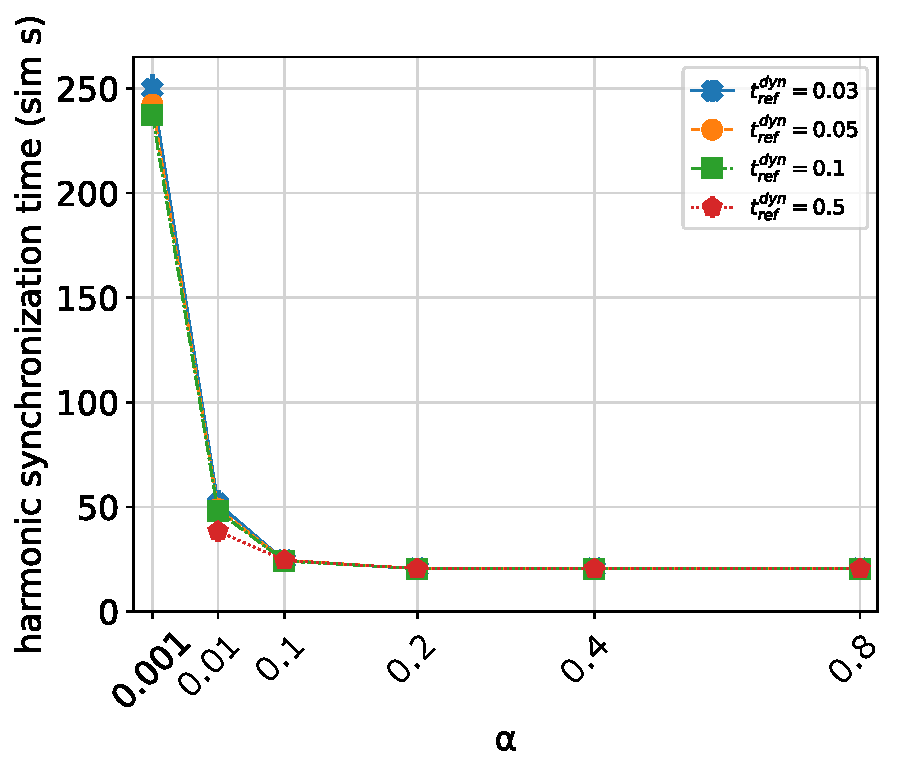
\includegraphics[width=\textwidth]{Assets/DocSegments/Chapters/ExperimentsAndResults/Figures/PerfScores/t_ref_dyn_x_alpha_hyperparamtuning_experiment_plot_collsize25.pdf}
			\caption{$|R|$ = 25.}
			\label{fig:sub:t_ref_dyn_x_alpha_collsize25}
		  \end{subfigure}
		  %
		  \begin{subfigure}[b]{0.5\textwidth}
			\centering\captionsetup{width=.9\linewidth}%
			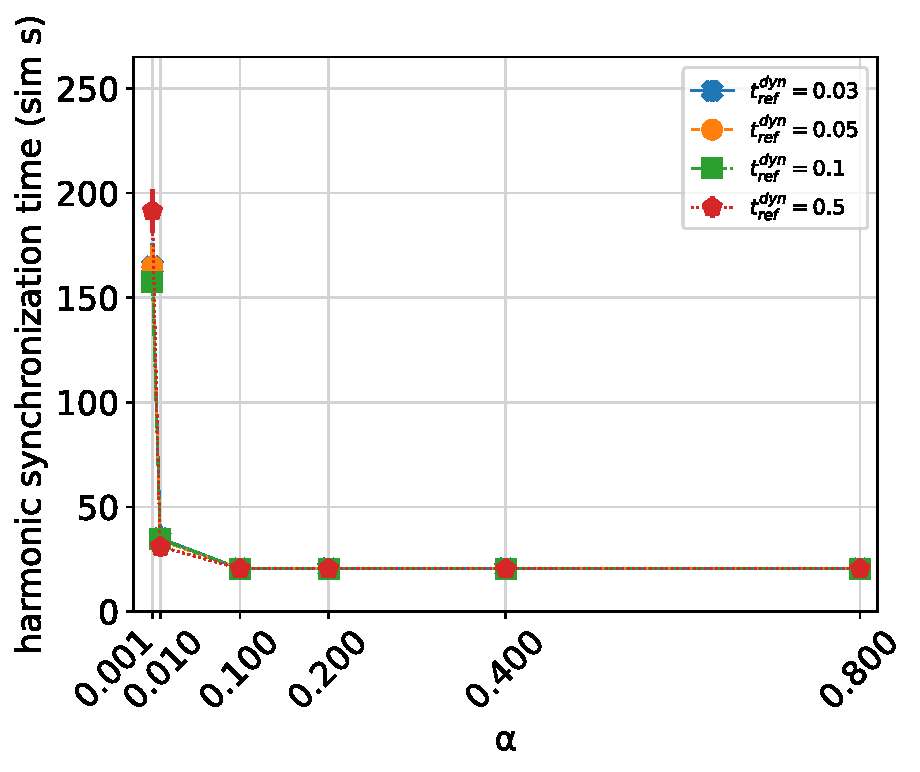
\includegraphics[width=\textwidth]{Assets/DocSegments/Chapters/ExperimentsAndResults/Figures/PerfScores/t_ref_dyn_x_alpha_hyperparamtuning_experiment_plot_collsize50.pdf}
			\caption{$|R|$ = 50.}
			\label{fig:sub:t_ref_dyn_x_alpha_collsize50}
		  \end{subfigure}
		  \caption{Average harmonic synchronization times are plotted in errorbar plots, where the standard deviation is the error. 30 simulation runs per $\alpha$ and $t_{ref}^{dyn}$ pair are reported, unless simulation runs ended up as ``synchronization fails.''}
		  \label{fig:phase_sync_hyperparam_tuning_experiment}
		\end{figure}
		
		As we can see in Figure \ref{fig:phase_sync_hyperparam_tuning_experiment}, there are generally low standard deviations which make errors in the plots barely visible. We also can notice that the largest differences are seen for lower $\alpha$ values, as average harmonic synchronization times are more and more overlapping and similar for larger $\alpha$ values.
		
		A general pattern we can see is that larger robot collective sizes (larger $|R|$ values) handle lower phase coupling constants $\alpha$ better; in that the music collectives both achieve harmonic synchrony in lower average times than the smaller robot collectives, as well as achieving lower error rates. To this latter point, note that for the lowest $\alpha$ value of 0.001, robot collectives with size $|R|=3$ and 10 were not able to achieve harmonic synchrony at all during any of the simulation runs (i.e. having 100\% error rate), whereas larger collective sizes like $|R|=25$ and $|R|=50$ managed to achieve harmonic synchrony despite the low $\alpha$ value. 
		
		\paragraph{Experiment analysis:\nl}
		
		The explanation for this latter observation regarding the seemingly increasing robustness with increasing collective sizes $|R|$ can very well lie in the fact that, as we remember, the phase coupling constant $\alpha$ represents how much each robot will adjust its phase when hearing a ''fire`` signal from a neighbouring robot. If there are more neighbours firing ``adjustment signals'' to a certain robot (i.e. we have a higher collective size $|R|$), it is also logical that the robot in question will update its phase more often. And so we can then see why e.g. all average harmonic synchronization times for $\alpha=0.01$ seem to improve (i.e. gets reduced) for every increase in collective size $|R|$; the phase coupling constant $\alpha=0.01$ might be weak, but with further and more frequent weak adjustments accumulated over the same time, the weak $\alpha$ is compensated for.
		
		Hence, it seems like larger robot collectives do not require as large of a phase coupling constant $\alpha$ in order to synchronize to each other compared to that which smaller robot collectives require.
	
	
	\subsection{Comparing phase adjustment methods}
	
		\paragraph{Experiment setup:\nl}
		
		So far in this chapter and section, we have only run experiments for pure phase synchronization, the $\phi$ problem, with Mirollo-Strogatz's method of phase adjustment, like described in \ref{mirollo_strogatz_phase_adjust}. With this method of phase synchronization, robots are simply adjusting phases in an excitatory way; they only ``push'' other ocillators's phases further or higher when firing themselves, never ``holding'' or ``dragging'' them back.
		
		Now, in order to investigate the validity of the claimed [] benefits of performing bi directional phase adjustments—both excitatory and inhibitory—like that of Nymoen's phase adjustment (see \ref{subsec:nymoen_phase_adjust}), an experiment comparing these two aforementioned phase adjustment methods thus follows.
		
		Empirically speaking based on previous results in phase synchronization experiments, in particular the ones shown in Figure \ref{fig:baseline_reproducing_phase_sync_for_alpha} and \ref{fig:phase_sync_hyperparam_tuning_experiment}, arguably the best values so far for $\alpha$ (i.e. $\alpha=0.8$) and $t_{ref}^{dyn}$ (i.e. $t_{ref}^{dyn}=0.1$) will be reused here for Mirollo-Strogatz's phase synchronization runs.
		
		Since we have not yet performed any experiments for pure phase synchronization in the $\phi$ problem using Nymoen's slightly modified and bi directional phase adjustment function, the same $\alpha$ value of 0.8 will also be used for the phase synchronization runs here.
		
		See the hyperparameter setup below in Table \ref{tab:directional_phase_adjustment_comparison}, and the results for the two phase adjustment methods given various robot collective sizes $|R|$ in \ref{fig:directional_phase_adjustment_comparison}. We here measure how long it takes various sizes of robot collectives to synchronize their phases to each other, given the two different phase adjustment methods.
		
		\begin{center}
		\begin{tabular}{ |c|c|c|c|c|c|c| } 
		\hline
		$\alpha$ & $\beta$ & $t_{ref}^{dyn}$ & $t_f$ & $k$ & $t_{max}$ \\
		\hline
		0.8 & 0 & 10\% & 80ms & 8 & 5min \\
		\hline
		\end{tabular}
		\captionof{table}{Experiment hyperparameter setup.}
		\label{tab:directional_phase_adjustment_comparison}
		\end{center}
		
		\paragraph{Experiment results:\nl}
		
		\begin{figure}[ht!]
		\begin{subfigure}[b]{0.5\textwidth}
			\centering\captionsetup{width=.9\linewidth}%
			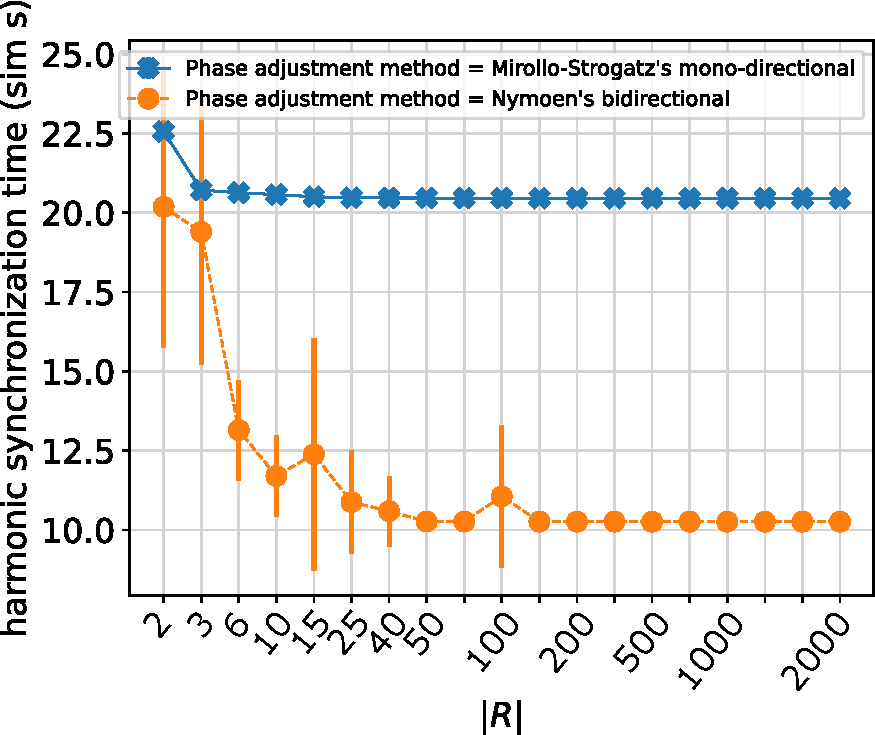
\includegraphics[width=\textwidth]{Assets/DocSegments/Chapters/ExperimentsAndResults/Figures/PerfScores/directional_phase_adjustment_comparison_hsynchtimes.pdf}
			\caption{Performance scores.}
			\label{fig:sub:directional_phase_adjustment_comparison_hsynchtimes}
		  \end{subfigure}
		  %
		  \begin{subfigure}[b]{0.5\textwidth}
			\centering\captionsetup{width=.9\linewidth}%
			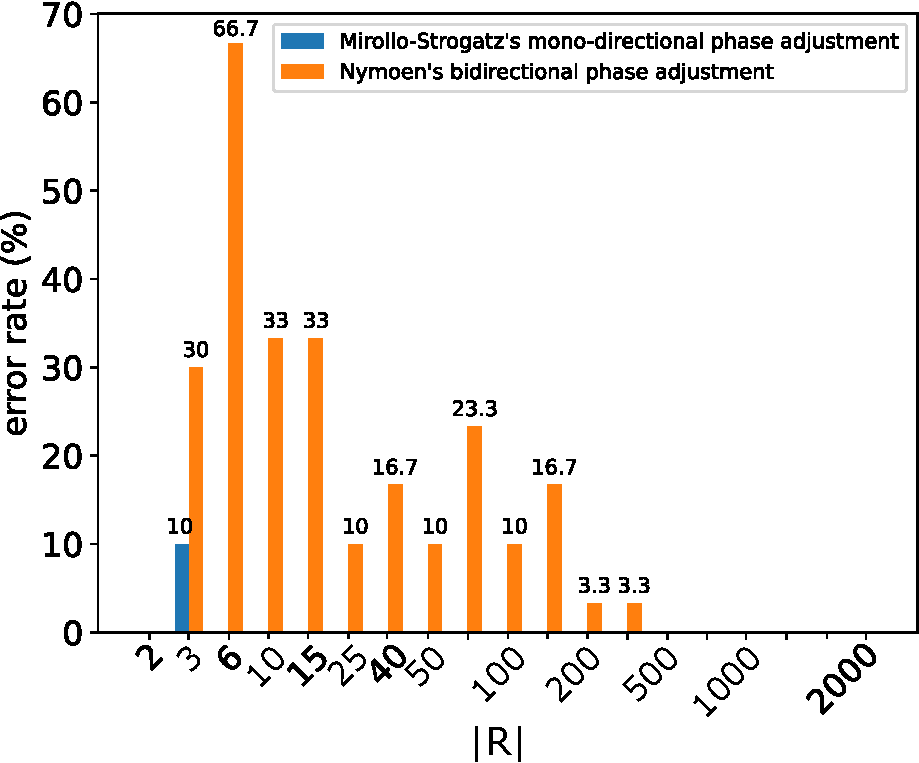
\includegraphics[width=\textwidth]{Assets/DocSegments/Chapters/ExperimentsAndResults/Figures/PerfScores/directional_phase_adjustment_comparison_errorRates.pdf}
			\caption{Error rates.}
			\label{fig:sub:directional_phase_adjustment_comparison_errorrates}
		  \end{subfigure}
		  \caption{Performance scores \ref{fig:sub:directional_phase_adjustment_comparison_hsynchtimes} given in average harmonic synchronization times (sim s) with standard deviation. Corresponding error rates in \ref{fig:sub:directional_phase_adjustment_comparison_errorrates} based on 30 individual runs per collective size $|R|$ for each of the two phase adjustment methods.}
		  \label{fig:directional_phase_adjustment_comparison}
		\end{figure}
		
		We quickly see from the results in Figure \ref{fig:directional_phase_adjustment_comparison} there seems to be a considerable difference in harmonic synchronization times between using Mirollo-Strogatz's and Nymoen's phase adjustment methods to synchronize phase in the phase ($\phi$) synchronization problem. In Subfigure \ref{fig:sub:directional_phase_adjustment_comparison_hsynchtimes}, we see that for smaller musical robot collectives $|R|$, differences in synchronization time on average are not especially large. However, as collective size $|R|$ increases, we see the harmonic synchronization times for Nymoen's bi directional phase synchronization becomes considerably lower than that of Mirollo-Strogatz's mono-directional on average, variance—or at least the square root of it—accounted for.
		
		On the other hand, when we look at the error rates in Subfigure \ref{fig:sub:directional_phase_adjustment_comparison_errorrates}, we also see that Nymoen's phase adjustment method's error rates are considerably higher than those of Mirollo-Strogatz's error rates (being nearly negligible). Interestingly, this is only the case until collective size $|R|=500$ though, after the point of which both phase adjustment methods's error rates are both equal to 0, and hence this objection towards Nymoen's phase adjustment method no longer holds. Hence, there seems to—at least up until $|R|=500$—exist a sort of tradeoff or high risk high reward scenario here, where one can in the phase ($\phi$) synchronization problem achieve harmonic synchrony faster by using Nymoen's phase adjustment method while at the same time risking a higher chance of the synchronziation failing; whereas Mirollo-Strogatz's method of phase adjustment on average seems to be the safer, albeit slower, option.
		
		Yet again, we also in these results notice a trend where smaller hyperparameter values lead to more unstable or worse performing synchronizations. Generally, although not strictly nor without exceptions, for both the harmonic synchronization times in Subfigure \ref{fig:sub:directional_phase_adjustment_comparison_hsynchtimes} and the error rates in \ref{fig:sub:directional_phase_adjustment_comparison_errorrates}, the larger the hyperparameter $|R|$, the more stable or quick synchronization runs we performed in the Unity synchronization simulator. 
		
		\paragraph{Experiment analysis:\nl}
		
		In this specific case, what this latter observation of seemingly increasing robustness given increasing collective sizes $|R|$ points to is perhaps that the system's robustness and stability is increasing as collective size increases—being a strength classically advocated for in the multi agent systems and swarm systems literature []; as well as being found in e.g. robustness degrees in networks where you in the one case have a single point of failure versus many redundant paths and edges between your nodes [].
		
		As we see, the synchronization simulator in Unity is able to synchronize with a lot of agents, still without having broken the simulation yet. Comparatively, Nymoen et al. \cite{nymoen_synch} only experimented with 6 oscillator nodes in their firefly system.
	

	\subsection{Increasing degree of self awareness}
	\label{exp:phasesync:increasing_SA_deg}
	
	So far in the harmonic synchronization experiments, we have only and by default used the most restrictive and comprehensive \textit{self awareness scopes}; all individual Dr. Squiggle robots have been globally connected, that is, and always hearing every neighbour Dr. Squiggle's fire signals. Now we want to challenge this strong connectivity assumption.
	
	Information and messages have the ability to travel through networks of many sorts, and the type of connectedness in these networks might influence how this occurs—and indeed the quality or accuracy of the travelled message; e.g. in a game of Chinese whispers versus a message sent through internet directly from the sender to the receiver. Both the speed as well as the overall quality of the message transmission can greatly be decided as a result of how connected the communicating nodes in a network are. Phenomena as these are to be experimented with here, as we will see how the connectedness between the musical Dr. Squiggle robots influence their collective and overall performance in synchronizing (harmonically).
	
	It has previously, although more mathematically and not so much experimentally, been attempted to reduce the connectivity assumptions in pulse coupled oscillators \cite{minimally_connected_pcos} and to analyze the effects of it.
	
	Here the hypothesis of whether increasing musical robots's degrees of self awareness will affect the synchronization performance or not, is investigated experimentally. Exactly what is meant by an increasing degree of self awareness specifically refers to the robots's \textit{self awareness scope} \cite{sacs17_ch3}. This is tested in Unity for the more challenging $\phi \& \omega$ problem of harmonically synchronizing both phases and frequencies. Perhaps a larger self awareness scope, meaning more knowledge about the social environment, will lead to the robots having a better ``overview'' of the environment; hence leading to shorter simulation time (s) before reaching the goal state of harmonic synchrony. Or perhaps hearing more ``fire'' signals on average simply will be disturbing to the robots and hence disturb and slow down their entrainment towards harmonic synchrony. This experiments attempts to answer questions like these by for the three \textit{self awareness scope} scenarios as introduced in \ref{SA_scopes_implemented} evaluating collective synchronization performance.
	
	
		\subsubsection{Self awareness scope tuning}
		\label{phase_sync_SA_scopes_tuning}

		In order to find out whether global connections in the pulse coupled oscillators is necessary to maintain performance in harmonic synchronization, varying \textit{self awareness scopes} (as introduced in \ref{SA_scopes_implemented}) are now experimented with.
		
			\paragraph{$k_s$ nearest neighbour scope\nl}
			
				\paragraph{Experiment setup:\nl}
				
				Firstly, the first \textit{self awareness scope} scenario (as in \ref{SA_scopes_implemented}) is experimented with and tuned for. The number of neighbouring Dr. Squiggle robots each individual Dr. Squiggle robot will listen for fire signals to ($k_s$) will be scaled and increased from $k_s=1$ up until $k_s=|R|-1$ which is the maximum number of neighbours each Dr. Squiggle robot can listen to for fire signals.

				In other words, the individual Dr. Squiggle robots's self awareness scope is increased incrementally in terms of \textit{$k_s$ nearest neighbour SA scope} and evaluated for performance in harmonic synchronization.

				Hyperparameters are set in the simulator as shown in Table \ref{tab:phase_sync_k_s_SA_scope_tuning}. Results can be seen in Figure \ref{fig:phase_sync_k_s_SA_scope_tuning}.

				\begin{center}
				\begin{tabular}{ |c|c|c|c|c|c|c| } 
				\hline
				$\alpha$ & $\beta$ & $t_{ref}^{dyn}$ & $t_f$ & $k$ & $t_{max}$ \\
				\hline
				0.8 & 0 & 10\% & 80ms & 8 & 5min \\
				\hline
				\end{tabular}
				\captionof{table}{Experiment hyperparameter setup.}
				\label{tab:phase_sync_k_s_SA_scope_tuning}
				\end{center}
				
				\paragraph{Experiment results:\nl}

				\tcol[blue]{FYLL INN}
				% \begin{figure}[ht!]
				% \begin{subfigure}[b]{0.5\textwidth}
					% \centering\captionsetup{width=.9\linewidth}%
					% \includegraphics[width=\textwidth]{Assets/DocSegments/Chapters/ExperimentsAndResults/Figures/PerfScores/}
					% \caption{Performance scores.}
					% \label{fig:sub:phase_sync_k_s_SA_scope_tuning}
				  % \end{subfigure}
				  % %
				  % \begin{subfigure}[b]{0.5\textwidth}
					% \centering\captionsetup{width=.9\linewidth}%
					% \includegraphics[width=\textwidth]{Assets/DocSegments/Chapters/ExperimentsAndResults/Figures/PerfScores/}
					% \caption{Error rates.}
					% \label{fig:sub:phase_sync_k_s_SA_scope_tuning}
				  % \end{subfigure}
				  % \caption{Performance scores \ref{fig:sub:phase_sync_k_s_SA_scope_tuning} given in average harmonic synchronization times (sim s) with standard deviation, given each nearest neighbour percentage $k_s/(|R|-1)$ for each $|R|$ and $k_s$ value pair. Corresponding error rates in \ref{fig:sub:phase_sync_k_s_SA_scope_tuning} based on 30 individual runs per collective size $|R|$ for each of the two phase adjustment methods.}
				  % \label{fig:phase_sync_k_s_SA_scope_tuning}
				% \end{figure}

				As we can see on the x axis in \ref{fig:sub:phase_sync_k_s_SA_scope_tuning}, we here plot harmonic synchronization scores per neighbour percentage $k_s/(|R|-1)$ which tells us the ratio of closest neighbours each robot listens to for fire signals out of all neighbours |R|-1 — or in other words the size of its self awareness scope, not given in absolute neighbours $k_s$.
		
				\paragraph{Experiment analysis:\nl}
				 
				 
			\paragraph{$d_s$ radial scope\nl}
	
	
		\subsubsection{Simulation breaking}
		
			\paragraph{Experiment setup:\nl}
			
			In order to test the limits of the developed synchronization simulator, we will here investigate the effects of scaling and exploding the musical robot collective size $|R|$—also given some various self awareness scopes found worthwhile to further investigate in the previous experiments in \ref{exp:phasesync:increasing_SA_deg}.
	
% --- \section END. ---



\section{Phase and frequency synchronization}
\label{sec:phase_and_freq_sync_experiments}
This is the section for the experiments attempting to synchronize for the second and harder problem of synchronizing both phases $\phi_i$, as well as frequencies $\omega_i$, for all agents $i$. These are then experiments where all musical robots originally have unequal and ever-changing phases  and frequencies, adjusting both phases and frequencies in order to entrain to synchronize their phases and frequencies until reaching harmonic synchrony. Or in other words, all experiments in this phase and frequency synchronization section have the two hyperparameters shown in Table \ref{tab:phase_and_freq_sync} in addition to the individual experiment hyperparameters listed.

\begin{center}
\begin{tabular}{ |c|c|c| } 
\hline
$Adj_\phi$ & $Adj_\omega$ \\
\hline
Nymoen & Nymoen  \\
\hline
\end{tabular}
\captionof{table}{Phase and frequency synchronization experiments hyperparameter setup.}
\label{tab:phase_and_freq_sync}
\end{center}



	\subsection{Initial validation}
	
	To see that synchronization is actually happening like intended, some relevant quantities and simulation values are recorded for a phase synchronization simulation run in Unity and displayed in \ref{}.
	
	\tcol[blue]{FYLL INN.}
	

	\subsection{Reproducing baseline results}
	Again, we want to here see whether we get more or less the same results in the Unity simulator as K. Nymoen et al. get in their firefly oscillator system.
	
	Hence, we here present attempts made in the novel Unity synchronization simulator at recreating K. Nymoen et al.'s first results with their novel frequency synchronization method, which is utilizing, amongst other aspects, self awareness \cite{nymoen_synch}.
	
		\subsubsection{Ordering by phase couplings}
		\label{exp:phase_and_freq_baseline_reproducing_initial_phase_ordering}
		
			\paragraph{Experiment setup:\nl}
			
			Given that K. Nymoen et al. do not mention their $\beta$ value in their frequency synchronization experiment where they order for different phase coupling values $\alpha$, an \textit{empirically decent} $\beta$ value of 0.4 is chosen for this experiment. What \textit{empirically decent} refers to in this case are K. Nymoen et al.'s findings in the results of their last experiment \cite{nymoen_synch} where synchronization times for various $\beta$ values were evaluated; deeming $\beta=0.4$ to be a good value, with no further improvement in synchronization performance when $\beta$ is increased further.
			
			Here, K. Nymoen et al.'s self aware frequency adjustment method, implemented in our novel synchrony simulator in Unity, is experimented with for varying phase coupling constants $\alpha$. This time not only oscillator phases are initially unsynchronized; oscillator frequencies are also unsynchronized to begin with. Hence, we here try to synchronize our musical robots in the phase ($\phi$) \textit{and} frequency ($\omega$) synchronization problem, using Nymoen's phase adjustment method to synchronize phases, as well as Nymoen's frequency adjustment method to synchronize frequencies. See set up hyperparameters in Table \ref{tab:baseline_reproducing_phase_and_freq_sync_for_alpha}. See the results in Figure \ref{fig:baseline_reproducing_phase_and_freq_sync_for_alpha}.
			
			\begin{center}
			\begin{tabular}{ |c|c|c|c|c|c|c|c|c|c| } 
			\hline
			$|R|$ & $\beta$ & $\omega_{min}^{init}$ & $\omega_{max}^{init}$ & $m$ & $t_{ref}$ & $t_f$ & $k$ & $t_{max}$ \\
			\hline
			6 & 0.4 & 0.5Hz & 4Hz & 5 & 50ms & 80ms & 8 & 5min \\
			\hline
			\end{tabular}
			\captionof{table}{Experiment hyperparameter setup.}
			\label{tab:baseline_reproducing_phase_and_freq_sync_for_alpha}
			\end{center}
			
			\paragraph{Experiment results:\nl}
			
			\begin{figure}[ht!]
				\centering
				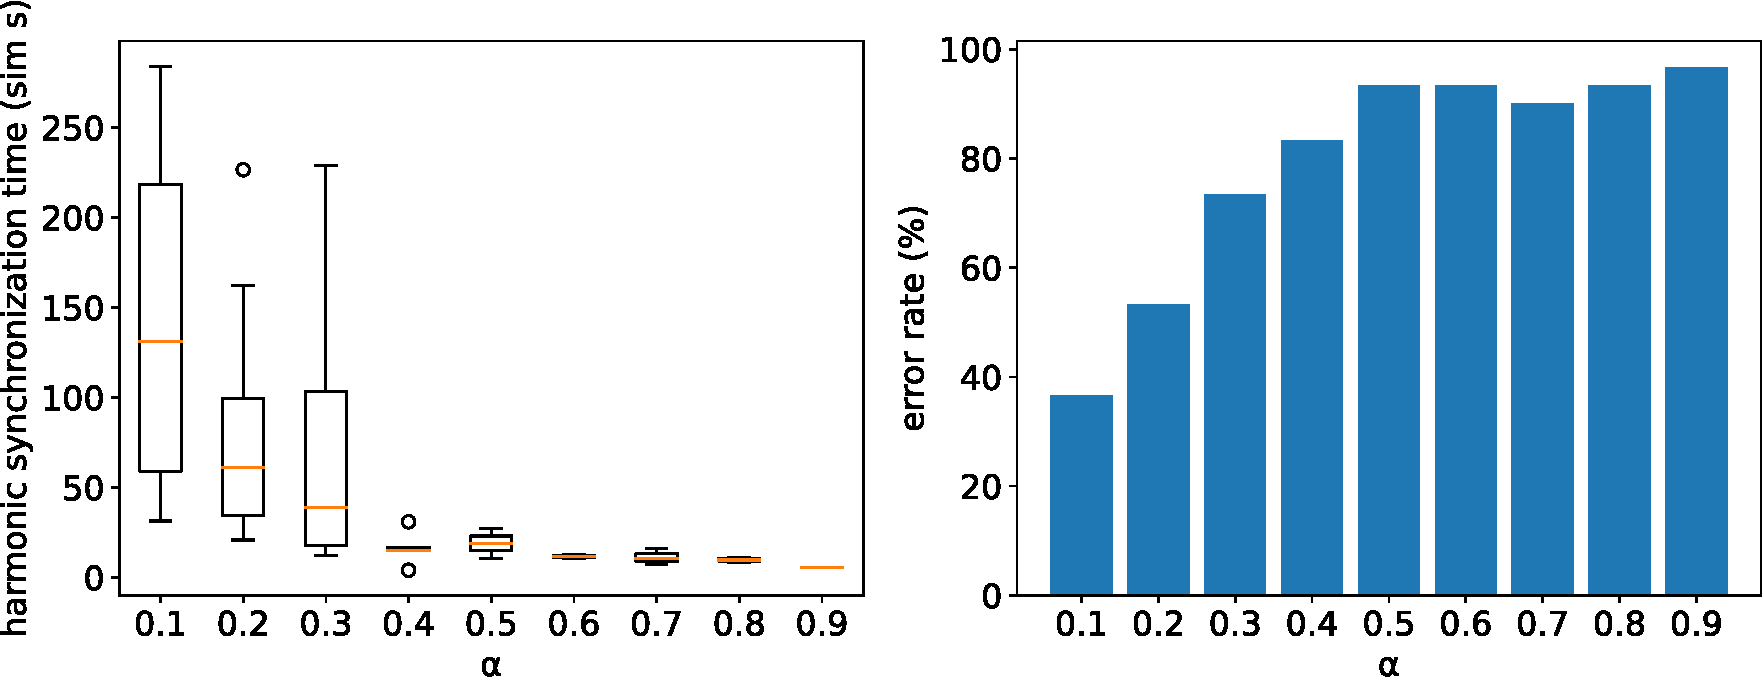
\includegraphics[width=\linewidth]{Assets/DocSegments/Chapters/ExperimentsAndResults/Figures/PerfScores/baseline_reproducing_phase_and_freq_sync_for_alpha.pdf}
				\caption{Harmonic synchronization times (sim s) for 6 robots with both initially unsynchronized phases \textit{and} frequencies, for varying phase coupling constants $\alpha$, reaching harmonic synchrony—but also often failing to. 30 simulation runs per $\alpha$ are reported.}
				\label{fig:baseline_reproducing_phase_and_freq_sync_for_alpha}
			\end{figure}
			
			\paragraph{Experiment analysis:\nl}
		
		
		\subsubsection{Ordering by phase couplings but with more stable hyperparameters}
		
			\paragraph{Experiment setup:\nl}
			
			After seeing how poorly the musical robot collectives managed to achieve harmonic synchrony during previous experiment \ref{exp:phase_and_freq_baseline_reproducing_initial_phase_ordering}, we change the hyperparameters slightly in the hopes of achieving harmonic synchrony more frequently, or in other words more stable synchronization simulation runs. The reason is mostly that it would be beneficial to actually see whether we observe similar patterns as in Nymoen's results—something which becomes impossible when robot collectives nearly never achieve harmonic synchrony.
			
			The frequency coupling constant of $\beta=0.6$ could potentially be another supposed good $\beta$ value, at least solely judging by Nomoen's results, and hence we select this value for this hopefully stable phase and frequency synchronization experiment.
			
			By initial trial and error, it also became apparent that phase \textit{and} frequency synchronization was not always stable—i.e. the robot collective not managing to achieve harmonic synchrony within the maximum time limit—for collective sizes of 6 or more. It did however become apparent that phase \textit{and} frequency synchronization \textit{was} stable for smaller musical robot collective sizes, like 2 or 3.
			
			Hence, a similar experiment to as in \ref{exp:phase_and_freq_baseline_reproducing_initial_phase_ordering} is set up in the Unity synchrony simulator, and is run similarly as before. So still, the phase ($\phi$) \textit{and} frequency ($\omega$) synchronization problem is to be experimented for, given different phase coupling constants $\alpha$, with Nymoen's both phase and frequency adjustment methods—only this time with $\beta=0.6$ and $collsize=3$ instead. See set up hyperparameters in Table \ref{tab:stable_baseline_reproducing_phase_and_freq_sync_for_alpha}. See results in Figure \ref{fig:stable_baseline_reproducing_phase_and_freq_sync_for_alpha}.
			
			\begin{center}
			\begin{tabular}{ |c|c|c|c|c|c|c|c|c|c| } 
			\hline
			$|R|$ & $\beta$ & $\omega_{min}^{init}$ & $\omega_{max}^{init}$ & $m$ & $t_{ref}$ & $t_f$ & $k$ & $t_{max}$ \\
			\hline
			3 & 0.6 & 0.5Hz & 4Hz & 5 & 50ms & 80ms & 8 & 5min \\
			\hline
			\end{tabular}
			\captionof{table}{Experiment hyperparameter setup.}
			\label{tab:stable_baseline_reproducing_phase_and_freq_sync_for_alpha}
			\end{center}
			
			\paragraph{Experiment results:\nl}
			
			\begin{figure}[ht!]
				\centering
				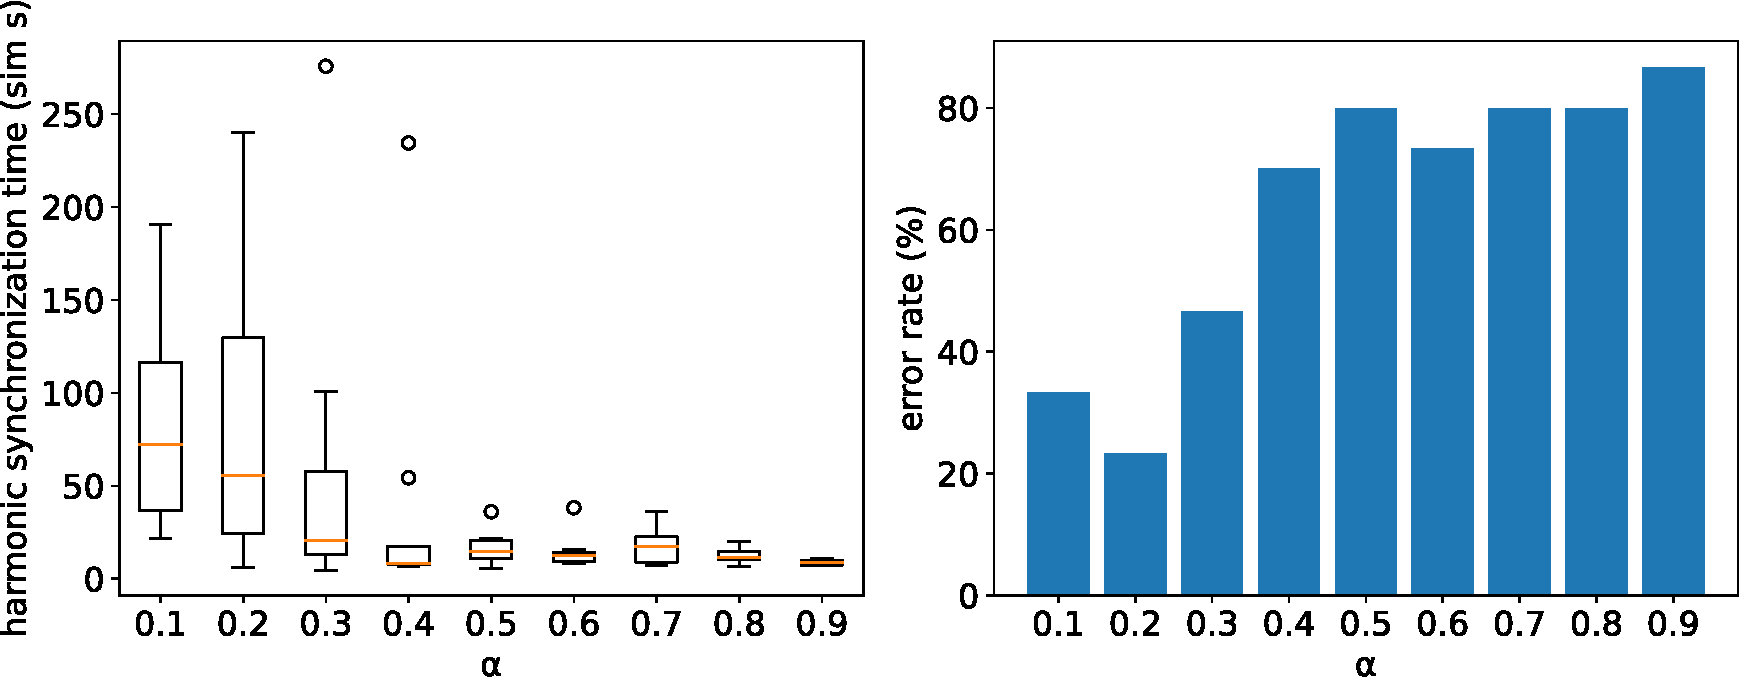
\includegraphics[width=\linewidth]{Assets/DocSegments/Chapters/ExperimentsAndResults/Figures/PerfScores/stable_baseline_reproducing_phase_and_freq_sync_for_alpha.pdf}
				\caption{Harmonic synchronization times (sim s) for 3 robots with both initially unsynchronized phases \textit{and} frequencies for varying phase coupling constants $\alpha$. 30 simulation runs per $\alpha$ are reported.}
				\label{fig:stable_baseline_reproducing_phase_and_freq_sync_for_alpha}
			\end{figure}
			
			\paragraph{Experiment analysis:\nl}
			
	
		\subsubsection{Ordering by frequency couplings}
		
		\paragraph{Experiment setup:\nl}
		
		Lastly, for the final Baseline reproducing experiment, it was wanted to see whether results within the phase and frequency ($\phi\&\omega$) synchronization problem, when one varied the frequency coupling constant $\beta$, also was more or less in the same ballpark or not, for the same reasons as mentioned in the first Baseline reproducing experiment in Section \ref{sec:phase_sync}.
		
		Since we now do not synchronize in Unity for varying phase coupling constants $\alpha$, we now fix $\alpha$ and rather test how the individual musical robots's various frequency coupling constants $\beta$ affect the performance of the musical robot collective.
		
		Again, Nymoen does not specify exactly the phase coupling constant $\alpha$ they use in their latter experiment when testing their firefly-inspired synchronization system for various $\beta$ values. Hence, the now fixed phase coupling constant $\alpha$ is here selected by reusing a reasonably good $\alpha$ value, based on the similar $\phi\&\omega$ synchronization experiments presented in Figure \ref{fig:baseline_reproducing_phase_and_freq_sync_for_alpha} and \ref{fig:stable_baseline_reproducing_phase_and_freq_sync_for_alpha}. In these two experiments in particular, $\alpha=2$ yielded both harmonic synchronization times among the best synchronization times, given the error scores; and furthermore, one of the lowest error rates. This then gives us a fixed $\alpha = 0.2$.
		
		See the set up hyperparameters for the experiment in Table \ref{tab:baseline_reproducing_phase_and_freq_sync_for_beta}, and the corresponding results in Figure \ref{fig:baseline_reproducing_phase_and_freq_sync_for_beta}.
		
		\begin{center}
		\begin{tabular}{ |c|c|c|c|c|c|c|c|c|c| } 
		\hline
		$|R|$ & $\alpha$ & $\omega_{min}^{init}$ & $\omega_{max}^{init}$ & $m$ & $t_{ref}$ & $t_f$ & $k$ & $t_{max}$ \\
		\hline
		6 & 0.2 & 0.5Hz & 4Hz & 5 & 50ms & 80ms & 8 & 5min \\
		\hline
		\end{tabular}
		\captionof{table}{Experiment hyperparameter setup.}
		\label{tab:baseline_reproducing_phase_and_freq_sync_for_beta}
		\end{center}
		
		\paragraph{Experiment results:\nl}
		
		\begin{figure}[ht!]
			\centering
			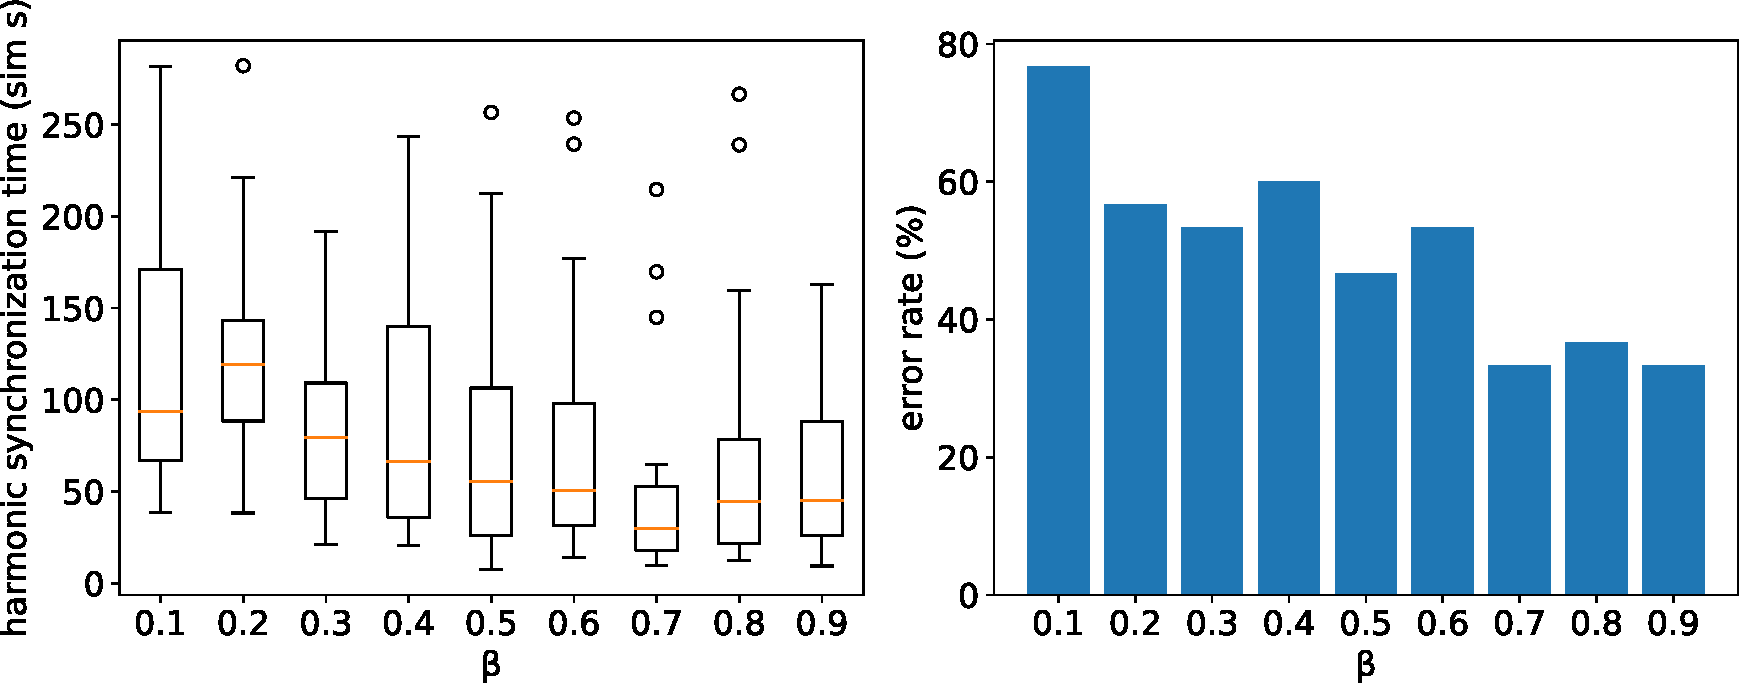
\includegraphics[width=\linewidth]{Assets/DocSegments/Chapters/ExperimentsAndResults/Figures/PerfScores/baseline_reproducing_phase_and_freq_sync_for_beta.pdf}
			\caption{Synchronization times (s) for 6 robots with both initially random and unsynchronized phases, and frequencies, for varying frequency coupling constants $\beta$. 30 simulation runs per $\beta$ are reported.}
			\label{fig:baseline_reproducing_phase_and_freq_sync_for_beta}
		\end{figure}
		
		Even though we do not see exactly the same harmonic synchronization times as we see in Nymoen's results, and worse at that, we do in fact see a similar pattern in that also here, synchronization times and error scores seem to improve the larger frequency coupling constant $\beta$ we have.
		
		\paragraph{Experiment analysis:\nl}
		
		Also, from the results in Figure \ref{fig:baseline_reproducing_phase_and_freq_sync_for_beta}, it becomes apparent that $\beta=0.7$ might be the best choice to continue using in our Unity synchrony simulator—at least when it comes to collective sizes $|R|=6$.
		
	
	\subsection{Increasing degree of self awareness}
	\label{exp:phase_and_freq_sync:increasing_SA_deg}
	
	Motivations and intentions are exactly the same as in \ref{exp:phasesync:increasing_SA_deg}, although now it is time to explore the effects of various degrees and scopes of self awareness in the second and more challenging phase and frequency ($\phi \& \omega$) synchronization problem.
	
		\subsubsection{Self awareness scope tuning}
		\label{phase_and_freq_sync_SA_scopes_tuning}
		
		Similarly to in the experiments in \ref{phase_sync_SA_scopes_tuning} we here want find out whether global connections in the pulse coupled oscillators really is necessary to maintain performance in harmonic synchronization, but for this time in the second and more complex ($\phi \& \omega$) synchronization problem.
		
			\paragraph{$k_s$ nearest neighbour scope\nl}
			
				\paragraph{Experiment setup:\nl}
			
				The first \textit{self awareness scope} scenario (as in \ref{SA_scopes_implemented}) is now again experimented with and tuned—only now for the phase and frequency ($\phi \& \omega$) synchronization problem. The number of neighbouring Dr. Squiggle robots each individual Dr. Squiggle robot will listen for fire signals to ($k_s$) will be scaled, for each $|R|$, and increased from $k_s=1$ up until $k_s=|R|-1$ which is the maximum number of neighbours each Dr. Squiggle robot can listen to for fire signals.
				
				In other words, the individual Dr. Squiggle robots's self awareness scope is increased incrementally in terms of \textit{$k_s$ nearest neighbour SA scope} and evaluated for performance in harmonic synchronization.

				Hyperparameters are set in the simulator as shown in Table \ref{tab:phase_and_freq_sync_k_s_SA_scope_tuning}. These are empirically found to be the best hyperparameters in previous experiment results in Section \ref{sec:phase_and_freq_sync_experiments} where we are attempting synchronization in the $\phi \& \omega$ problem.
				
				Results can be seen in Figure \ref{fig:phase_and_freq_sync_k_s_SA_scope_tuning}.

				\begin{center}
				\begin{tabular}{ |c|c|c|c|c|c|c| } 
				\hline
				$\alpha$ & $\beta$ & $t_{ref}^{dyn}$ & $t_f$ & $k$ & $t_{max}$ \\
				\hline
				0.2 & 0.7 & 10\% & 80ms & 8 & 5min \\
				\hline
				\end{tabular}
				\captionof{table}{Experiment hyperparameter setup.}
				\label{tab:phase_and_freq_sync_k_s_SA_scope_tuning}
				\end{center}

				\paragraph{Experiment results:\nl}
				
				\tcol[blue]{FYLL INN}
				% \begin{figure}[ht!]
				% \begin{subfigure}[b]{0.5\textwidth}
					% \centering\captionsetup{width=.9\linewidth}%
					% \includegraphics[width=\textwidth]{Assets/DocSegments/Chapters/ExperimentsAndResults/Figures/PerfScores/}
					% \caption{Performance scores.}
					% \label{fig:sub:phase_and_freq_sync_k_s_SA_scope_tuning}
				  % \end{subfigure}
				  % %
				  % \begin{subfigure}[b]{0.5\textwidth}
					% \centering\captionsetup{width=.9\linewidth}%
					% \includegraphics[width=\textwidth]{Assets/DocSegments/Chapters/ExperimentsAndResults/Figures/PerfScores/}
					% \caption{Error rates.}
					% \label{fig:sub:phase_and_freq_sync_k_s_SA_scope_tuning}
				  % \end{subfigure}
				  % \caption{Performance scores \ref{fig:sub:phase_and_freq_sync_k_s_SA_scope_tuning} given in average harmonic synchronization times (sim s) with standard deviation. Corresponding error rates in \ref{fig:sub:phase_and_freq_sync_k_s_SA_scope_tuning} based on 30 individual runs per collective size $|R|$ for each of the two phase adjustment methods.}
				  % \label{fig:phase_and_freq_sync_k_s_SA_scope_tuning}
				% \end{figure}

				\paragraph{Experiment analysis:\nl}
			
			
			\paragraph{$d_s$ radial scope}
	
	
		\subsubsection{Simulation breaking}
		
			\paragraph{Experiment setup:\nl}
			
			In order to test the limits of the developed synchronization simulator, we will here investigate the effects in harmonic synchronization performance when scaling and exploding the musical robot collective size $|R|$—also given some various self awareness scopes found worthwhile to further investigate in the previous experiments in \ref{exp:phase_and_freq_sync:increasing_SA_deg}.
	
% --- \section END. ---